% displayname : Division du front d'onde
\documentclass[12pt,fancy]{cours}
\Chapit{3}{3}
\begin{document}
\maketitre{
Nous avons discuté des conditions nécessaires à l'obtention d'interférences (polarisation non orthogonales, accord de fréquence et de phase) ; en particulier,  la condition d'accord de phase est presque impossible à réaliser en pratique à partir de deux sources indépendantes: on cherchera donc à créer deux sources secondaires à partir d'une source unique. Dans ce chapitre nous étudions un premier type d'interféromètre dit à division du front d'onde, qui opère une division géométrique du faisceau incident. Dans le cadre du programme, nous nous focalisons sur le dispositif interférentiel des trous de Young proposé par T. Young en 1801. Nous allons maintenant exprimer la différence de marche $\delta(M)$ qui intervient dans l'expression de l'intensité $I(\delta)$  vue au chapitre précédent et en déduire les propriétés de la figure d'interférences. On pourra trouver des animations sur le lien suivant : \href{https://xyod.github.io/anim-ophy/Young/}{https://xyod.github.io/anim-ophy/Young/}.
}
{
\item Cours Signaux 2 - 0
\item Document de cours Signaux 2 - 1 à 3
\item TD Signaux 2
}



% http://anim.institutoptique.fr/

%%%%%%%%%%%%%%%%%%%%%%%%%%%%%%%%%%%%%%%%%%%%%%%%%%%%%%%%%%%%%%%%%%%%%%%%%%
\section{Le dispositif des trous de Young}
\label{sec:young}

En raison de la condition d'accord de phase, deux ondes ne peuvent être cohérentes que si elles proviennent d’une \emph{même source}. Il faut donc former deux sources secondaires $S_1$ et $S_2$ à partir d'une source unique. Il existe deux types de dispositif pour produire ces interférences. Nous nous intéressons dans ce chapitre à la \imp{division du front d’onde} : le front d’onde issu d’une source primaire $S$ est divisé géométriquement en deux faisceaux, créant ainsi des secondaires $S_1$, $S_2$, etc. séparées dans l’espace. Le dispositif canonique de division du front d’onde est celui des \imp{trous d’Young}, qui produit une interférence à deux ondes.

\begin{definition}[Division du front d'onde]\label{def:}
  Un interféromètre à division du front d'onde opère une \imp{division géométrique} du front d'onde issu d'une source primaire $S$ en plusieurs fronts d'onde secondaires qui interfèrent en un point $M$. L'exemple canonique est les \imp{trous de Young}.
\end{definition}




\subsection{Schéma de l'expérience}
Le dispositif est schématisé en \Fig{schema_young}, et contient les éléments suivants.
\begin{liste}
  \item Une  \imp{source ponctuelle monochromatique} $\rm S$ sur l’axe optique $(Oz)$.
  \item Deux \imp{trous} $\rm S_1$ et $\rm S_2$ séparés de $a$ placés \imp{symétriquement} sur l’axe optique.
  \item Un \imp{écran} placé à une distance $D$ en aval des trous, où se forme la figure d'interférences.
\end{liste}
%La dénomination de division du front d'onde se comprend en représentant les surfaces d'onde (pointillés orange):
% La lumière incidente diffracte au niveau des trous, qui se comportent comme des sources secondaires $\rm S_1$ et $\rm S_2$, et réémettent des fronts d’ondes cohérents. 

%Une même surface d'onde de l'onde initiale est géométriquement séparée en deux, puis ces deux parties distinctes

%%%%%%%%%%%%%%%%%%%%%%%%%%%%%%%
\begin{figure}[H]
  \centering
  
\includegraphics[width=\textwidth]{experience_young_simple.pdf}
  \caption{Schéma du dispositif des trous de Young. Une source ponctuelle $S$ éclaire deux trous centrés par rapport à l'axe optique, séparés d'une distance $a$. Par le phénomène de diffraction, ces deux trous se comportent comme deux sources secondaires $S_1$ et $S_2$ qui émettent deux onde sphériques en phase qui interférent en un point $M(x,y)$ d'un écran placé à grande distance $D\gg a$. [Source : femto-physique].  
  % Les trous de Young vus de face sont représentés dans le coin supérieur gauche: leur diamètre est négligeable devant la distance qui les sépare ($\varepsilon\ll a$).
  %Typiquement $a\sim\SI{1}{mm}$ et $\varepsilon\sim\SI{0.1}{mm}$.
  }
  \label{fig:schema_young}
  \end{figure}
 %%%%%%%%%%%%%%%%%%%%%%%%%%%%%%%%%

 
 La superposition des d’ondes sur l’écran est possible grâce à la \imp{diffraction} de la lumière par chacun des trous, qui agissent comme deux sources secondaires émettant deux faisceaux élargis. La région ou se superposent les faisceaux provenant des trous est appelée \imp{champ d'interférences}, voir \Fig{champ_interf}. Il s'agit ici d'une région étendue spatialement, ce qui est le cas de tous les dispositifs à division du front d'onde. On dit que les interférences sont \imp{délocalisées}.
 
\begin{prop}[Champ d’interférences]
  Dans un interféromètre à division du front d'onde, les rayons interférent dans une région étendue de l'espace appelée \important{champ d'interférences}. On dit que les interférences sont \imp{délocalisées}.
\end{prop}

\begin{figure}[H]
  \centering
  \subfigure[]{\label{fig:champ_interf}
  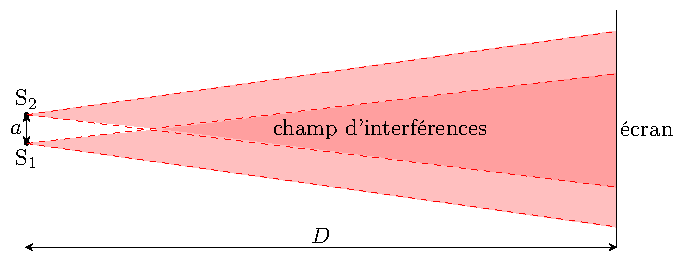
\includegraphics[height=5cm]{Figures/champ_interfer.pdf}
  }
  \subfigure[]{\label{fig:interf_young}
  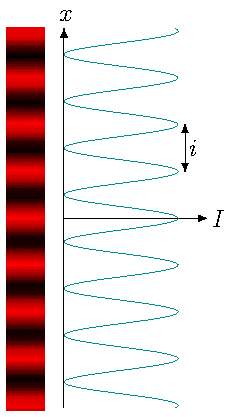
\includegraphics[height=5cm]{Figures/figure_interf_young.pdf}
  }
  \caption{(a) Champ d'interférences des trous de Young. (b) Figure d'interférences des trous de Young. On pourra visualiser une animation de la formation de la figure d'interférences ici : \href{https://femto-physique.fr/simulations/young-experience.php}{https://femto-physique.fr/simulations/young-experience.php}.}
  % \label{fig:champ}
\end{figure}


\begin{exemple}{Champ d'interférences des trous de Young}
   On a représenté le champ d'interférences des trous de Young sur la \Fig{champ_interf}. 
  \begin{quest}
    \item	Rappeler l’expression de l’ouverture angulaire $\theta$ du faisceau diffracté par un trou de diamètre $d$.
    \item	Exprimer la taille $L$ du champ d'interférences pour $D\gg a$. \AN~pour $D\simeq \SI{1}{m}, d\simeq \SI{100}{\mu m}$ et une lumière dans le vide de longueur d’onde $\lambda \simeq \SI{500}{nm}$. 
  \end{quest}
 
  % Le faisceau issu de la diffraction en sortie de chaque source secondaire est de largeur angulaire $\theta\sim \frac{\lambda}{d}$ où $d$ représente le diamètre des trous. 
\end{exemple}
\examplesol{
  \begin{quest}
    \item	L’ouverture angulaire du faisceau diffracté par un trou de diamètre $d$ est donnée par la relation .
    \eqbox{
    \theta \simeq \frac{\lambda}{d}.
    }
    \item   La largeur du champ d'interférences est donc de l'ordre de 
    \eqbox{
    L\simeq 2 \theta D \simeq \frac{2 \lambda D}{d}.
    }
    \AN~: $L \simeq \SI{1}{cm}$. C’est une région relativement réduite de d’écran !
  \end{quest}

}

\subsection{Figure d’interférences}\label{subsec:expression_delta}
Dans le chapitre précédent, nous avons montré que l’intensité lumineuse issue de l'interférence de deux ondes cohérentes monochromatiques de longueur d'onde dans le vide $\lambda_0$ et de même intensité $I_0$ s’écrit
% \begin{equation}\label{eq:fresnel_simple}
\eqbox[fresnel_simple]{
  I(M)= 2I_0\left[1 + \cos\left(2\pi \frac{\delta(M)}{\lambda_0}\right)\right].
  }
% \end{equation}
Pour déterminer le profil d'intensité lumineuse $I(M)$ sur l'écran pour une source, il reste à exprimer $\delta(M)$. Pour simplifier, nous assimilons l’air au vide, d’indice de réfraction $n =1$, et nous supposons que le point M$(x,y=0)$ est placé sur l’axe $x$ de l’écran, dans le plan du tableau.
\parag{Calcul de la différence de marche} À un signe global près, on a
\begin{equation}
\delta(M) = \opt{S M}_1-\opt{S M}_2 = [ \opt{SS_1} +  \opt{S_1 M} ] + [ \opt{S_2 M} - \opt{S_1 M} ] = \opt{S_2 M}-\opt{S_1 M} = S_2M-S_1M,
\end{equation}
car $\opt{SS_1} = \opt{SS_2}$ par symétrie : la source est équidistante des deux trous.

Notons $\rm O$ l'origine de l'axe $x$ sur l'écran, situé sur l'axe optique, et $\rm H_1$ et $\rm H_2$ les projetés orthogonaux de $\rm S_1$ et $\rm S_2$ sur l'écran. On a alors d'après le théorème de Pythagore,
\begin{equation}
  \begin{cases}
      S_1 M^2 & = S_1H_1^2 +H_1M^2 = D^2 + (x + \frac{a}{2})^2 = D^2 + \left(\frac{a}{2}\right)^2+x^2 +ax \\ 
      S_2 M^2 & = S_2H_1^2 +H_2M^2 = D^2 + (x - \frac{a}{2})^2 = D^2 + \left(\frac{a}{2}\right)^2+x^2-ax
  \end{cases}
  \end{equation}
En pratique, il est légitime de supposer que l'écran est loin des trous et que sa distance est grande devant la largeur du champ d’interférences, i.e. $D \gg a,x,y$.
\begin{prop}[Approximation paraxiale]%\label{prop:}
Les rayons interférant en un point $\rm M$ de l'écran sont peu inclinés par rapport à l’axe optique, soit
$$D \gg a,x,y.$$
\end{prop}
 Au premier ordre, on a le développement limité
\begin{equation}
S_1 M = D\sqrt{1+\underbrace{\left(\frac{a}{2D}\right)^2+\dfrac{x^2 -ax}{D^2}}_{\veps \ll 1}}\simeq D\left(1 +\frac{\veps}{2}\right) = D + \dfrac{a^2+4x^2}{8D}-\frac{ax}{2D},
\end{equation}
On montre de la même manière que
\begin{equation}
S_2 M\simeq D+\dfrac{a^2+4x^2}{8D}+\frac{ax}{2D}.
\end{equation}
La différence de marche vaut donc
\eqbox[]{
  \label{eq:deltaM}
  \delta(M)\simeq\frac{ax}{D}
}  

\parag{Figure d’interférences} En utilisant la formule de Fresnel \Eq{fresnel_simple}, on trouve
\begin{equation}\label{eq:I_young}
I(x)=2I_{0}\left[1+\cos\left(2\pi \frac{a x}{\lambda_0 D}\right)\right].
\end{equation}
En généralisant à un point $M$ décalé de $y$, et à un milieu d’indice $n$, on obtiendrait,
\begin{equation}
I(x,y)=2I_{0}\left[1+\cos\left(2\pi \frac{a x}{\lambda D}\right)\right],
\end{equation}
où $\lambda = \lambda_0/n$ est la longueur d’onde dans le milieu.
L'intensité sur l’écran ne dépend donc pas de $y$, ce qui est cohérent en raison de la symétrie du dispositif. La figure d’interférences est ainsi composé de \important{franges rectilignes} dans la direction $y$, alternativement sombres et brillantes (Fig.~\ref{fig:interf_young}). Ces fentes sont régulièrement espacées et séparées d'une distance $i$ appelée \imp{interfrange}.

L'interfrange correspond à la période spatiale de la figure d'interférences, et donc à la période spatiale du cosinus dans l’\Eq{I_young}. On peut donc mettre l’intensité sous la forme
\eqbox[]{
  I(x)=2I_{0}\left[1+\cos\left(2\pi\frac{x}{i}\right)\right],
  }
d’où l’on tire $i=\frac{\lambda D}{a}$. Dans le cas général, on peut utiliser la méthode suivante.
\begin{methode}[Déterminer un interfrange]
  \item	Déterminer l’\imp{ordre d’interférences} $p(x)$.
  \item Écrire que la \imp{décalage} entre deux franges successives vérifie $p(x+i) - p(x) = 1$.
\end{methode}
% trouver l'interfrange en écrivant que $p(x+i)=p(x)+1$ ou $p=\frac{\delta}{\lambda}$ désigne l'ordre d'interférence, qui est entier pour une frange brillante. En généralisant à un milieu homogène d’indice optique $n$, on remplace la longueur d'onde dans le vide $\lambda_0$ par la longueur d'onde dans le milieu $\lambda=\frac{\lambda_0}{n}$.
\begin{theorem}[Figure d’interférences des trous de Young]%\label{form:}
  La figure d’interférences des trous de Young est constituée de \imp{franges rectilignes} transverses à l’axe des trous séparées d’une distance constante, appelée
    \imp{interfrange}, d’expression
  \begin{equation*}
  i=\frac{\lambda D}{a}.
\end{equation*}
\end{theorem}
% \noindent avec $\lambda=\frac{\lambda_0}{n}$ la longueur d’onde dans le milieu.


% \begin{exemple}{Ordre de grandeur}
% On souhaite obtenir un interfrange d'environ \SI{1}{mm} en plaçant un écran à \SI{20}{cm} des trous de Young et en utilisant comme source un faisceau laser He-Ne rouge à \SI{632.8}{nm}. De quelle distance $a$ sont séparés les trous?

% \end{exemple}
% \examplesol{
%   On obtient dans l'air $a=\lambda_0 D/i\simeq\SI{0.1}{mm}$, ce qui est proche. C'est pour cela que les interférences ne sont pas si faciles à observer!
% }

\begin{experience}{Mesure d’un interfrange}\label{exp:}
  En plaçant un écran à une distance $D=\SI{150}{cm}$ des trous de Young séparés d'une distance $a=\SI{200}{\micro m}$, et éclairé par une diode laser de longueur d’onde $\lambda \simeq \SI{650}{nm}$, on trouve un interfrange $i\simeq \SI{5}{mm}$. 
\end{experience}


\subsection{Montage de Fraunhofer}

\parag{Principe}
L'interférence par les trous de Young a été étudiée dans l'approximation paraxiale, qui exige que l'écran soit loin des trous. Mais plus l'écran est loin, plus la luminosité est faible. Pour s'affranchir de cette contrainte, on utilise le \imp{montage de Fraunhofer}, qui contient deux lentilles convergentes.
 % Le montage permet d'agrandir l’image avec un doublet de lentilles, tout en ayant une bonne luminosité. Le schéma est représenté en Fig.~\ref{fig:young_fraunhofer}. La source et l'écran sont respectivement dans le plan focal objet et image des lentilles 1 et 2, : elles transforment les ondes sphériques en ondes planes.
\begin{enumerate}
  \item On simule une \imp{source à l'infini} en plaçant $S$ au foyer objet d'une lentille $\mc{L}_1$.
  %La condition $D \gg a$
    \item On simule un \imp{écran à l'infini} en le plaçant dans le plan focal image d'une lentille $\mc{L}_2$. 
    %  La condition $D \gg a,x,y$ est alors rigoureusement vérifiée.
\end{enumerate}
Le faisceau lumineux est donc parallèle entre les deux lentilles, ce qui permet de placer les trous à notre guise sans modifier la figure d’interférences. La figure d’interférences n’est pas non plus modifiée si l’on déplace l’écran et la lentille $\mc{L}_2$ ensemble.
\begin{prop}[Intérêt du montage de Fraunhofer]
  Le montage de \imp{Fraunhofer} permet d'obtenir des interférences avec une \imp{bonne luminosité}.
\end{prop}


 \begin{figure}[H]
 \centering
 
\includegraphics[width=\textwidth]{fraunhofer.pdf}
 \caption{Montage de Fraunhofer pour l'expérience des trous de Young. Bien noter que la source est dans le plan foyer objet de la première lentille et l'écran dans le plan foyer image de la seconde. En appliquant le théorème de Malus pour les deux rayons en rouge, leur différence de marche est donnée par $\opt{S_2 H}$.}
 \label{fig:young_fraunhofer}
 \end{figure}

\parag{Différence de marche}
Calculons la différence de marche dans cette nouvelle configuration. Les faisceaux interférant en $M$ sont parallèles avant et après les trous. D’après le théorème de Malus, le plan d’onde passant par $\rm S_2$ est orthogonal aux rayons lumineux. Soit $\rm H$ l’intersection du rayon $1$ et du plan d’onde passant par $\rm S_2$. On a donc 
\begin{equation}
  \vphi(H) = \vphi(S_2) \Rar \opt{S_2 M} = \opt{HM},
\end{equation}
en vertu de la formule du déphasage. Par additivité, et en supposant que le milieu est de l'air d'indice $n=1$, 
\begin{equation}
\delta(M)=  \opt{S_1 M}-\opt{S_2 M}= [\opt{S_1H} + \opt{HM}] - \opt{S_2 M} = \opt{S_1H} =  a \sin\theta,
\end{equation}
où l’angle $\theta$ est représenté sur la \Fig{young_fraunhofer}. Or cet angle se retrouve également entre les rayons lumineux et l’axe optique, et donc 
\begin{equation}
  \tan \theta = \frac{x}{f'_2}.
\end{equation}
Dans les conditions de Gauss, $\sin(\theta) \simeq \tan(\theta)$, et on déduit que
% \begin{equation}
\eqbox[]{
  \delta(x)=\frac{ax}{f'_2}.
  }
% \end{equation}
On trouve la même expression qu’en \Eq{deltaM}, sauf que la distance à l’écran $D$ est remplacée par la distance focale $f'_2$. L’interfrange vaut donc 
\begin{equation}
i = \frac{\lambda f'_2}{a}.
\end{equation}
En pratique, les distances focales usuelles sont inférieures au mètre, ce qui conduit à une image plus petite que dans le montage classique, mais on gagne en luminosité.

% Si l'on prend une grande distance focale ($\sim\SI{1}{m}$), l'interfrange $i=\frac{\lambda f'_2}{a}$ est tout aussi grand qu'en plaçant un écran lointain tout en conservant une bonne luminosité, puisque le faisceau est collimaté.

\begin{prop}[Interfrange dans le montage de Fraunhofer]
  % Le montage de \imp{Fraunhofer} permet d'obtenir des interférences avec une \imp{bonne luminosité}. 
  Dans les conditions de Gauss, l'interfrange dans le montage de Fraunhofer  vaut
  $$
  i =\frac{\lambda f'_2}{a}.
  $$
\end{prop}

\section{Perte de contraste}

Dans le modèle présenté dans la \Sec{young}, les interférences sont parfaitement contrastées (contraste $\mc{C}=1$). Dans la réalité, plusieurs phénomènes limite la visibilité des interférences. Nous allons en discuter deux : l'élargissement spectral de la source et le problème associé de cohérence temporelle ; et l'élargissement spatial de la source et le problème associé de cohérence spatiale. 


\subsection{Élargissement spectral de la source et cohérence temporelle}

%%%%%%%%%%%%%%%%%%%%%%%%%%%%%%%%
 \begin{figure}[b!]
 \centering
 \subfigure[]{\label{fig:couleur_young}
 
\includegraphics[height=7.5cm]{3lumieres_young.png}
 }
  \subfigure[]{\label{fig:blanc_young}
 
\includegraphics[height=7.5cm]{blanc_young.png}
 }
 \caption{(a) Pour 3 longueurs d'onde différentes (bleu à \SI{450}{nm}, vert à \SI{532}{nm} et rouge à \SI{633}{nm}) on peut constater que l'interfrange (repéré par les traits blancs pointillés) augmente avec la longueur d'onde. (b) La lumière blanche étant une superposition de toutes les couleurs du visible, on observe au centre de la figure d'interférences en lumière blanche une frange blanche entourée de franches noires (les cannelures). Puis, comme l'interfrange dépend de $\lambda$, on observe un chevauchement des ordres d'interférences et donc des irisations progressives (les teintes de Newton). Lorsque la différence de marche devient trop importante, on obtient le blanc d'ordre supérieur qui comporte de très nombreuses cannelures invisibles à l’œil nu. Lien YouTube: \href{https://youtu.be/tc6V9B7YjtU}{https://youtu.be/tc6V9B7YjtU}.}
 \label{fig:lumiere_blanche_young}
 \end{figure}
%%%%%%%%%%%%%%%%%%%%%%%%%%%%%%%%%%%%%

Que se passe-t-il si l'on éclaire les trous de Young avec une source polychromatique, par exemple en lumière blanche. Rappelons ce que nous avons vu au chapitre précédent. 
La comparaison entre la différence de marche $\delta$ entre les deux ondes issues de la même source et la longueur de cohérence permet de savoir si elles peuvent interférer.

\begin{liste}
\item Lorsque $\delta \lesssim l_{\rm{c}}$,  deux trains d'onde qui se recouvrent ont la même phase et interfèrent donc constructivement. Les ondes sont \imp{cohérentes}.

\item Lorsque $\delta \gtrsim  l_{\rm{c}}$, le déphasage entre les trains d'ondes conduit à des interférences destructives et donc un brouillage de la figure d'interférences. Les ondes sont \imp{incohérentes}.
\end{liste}
% \begin{remarque}
% Cela explique la facilité d'obtention des interférences avec un laser: comme celui-ci a une longueur de cohérence temporelle $\lc \sim \SI{30}{cm}$ de l’ordre de grandeur de la taille d’un montage optique, on peut observer les interférences sur une large plage de différence de marche.
% %, ce qui simplifie le réglage.
% \end{remarque}
Le cas limite s'obtient lorsque $\delta \simeq \lc$, c'est-à-dire lorsque l'ordre d'interférences vaut $p=\frac{\delta}{\lambda} \simeq \frac{\lc}{\lambda}$. La longueur de cohérence temporelle donne donc une estimation du nombre de franges visibles dans le champ d'interférences,
\begin{equation}
  N_{\rm{f}}\simeq \frac{\lc}{\lambda}\simeq\frac{\lambda}{\Delta\lambda}.
  \end{equation}
Pour un source de lumière blanche, on obtient $N_{\rm f}$ de l'ordre de l'unité : on ne peut observer qu'un petit nombre de franges d'interférences. 

C'est ce que l'on observe sur la \Fig{blanc_young}, où l'on voit que la frange centrale est blanche, entourée de franges noires et de franges colorées. Interprétons. L'interfrange $i = \lambda D/a$ dépend de la longueur d'onde $\lambda$, ce qui peut se vérifier expérimentalement avec plusieurs lasers (Fig.~\ref{fig:couleur_young}). La lumière blanche, c’est-à-dire une superposition de toutes les couleurs du visible, entre $\SI{400}{nm}$ et $\SI{750}{nm}$. Chaque couleur produit sa propre figure d’interférences, et les intensités associées à différentes couleurs, qui sont incohérentes entre elles, s’additionnent.
\begin{liste}
  \item La frange centrale correspond à $\delta=0$ quelle que soit la longueur d’onde. Toutes les franges centrales colorées se superposent, et donc la frange centrale reste brillante et apparaît blanche.
  \item Pour des différences de marche $\delta \neq 0$, les franges brillantes de chaque couleur sont décalées, ce qui conduit à une alternance de couleurs puis à une perte de visibilité pour les grandes différences de marche, où les franges colorées sombres et brillantes se chevauchent.
  %  C’est bien ce qu’on observe sur la figure d'interférences de la Fig.~\ref{fig:blanc_young}.
\end{liste}
Quantitativement, la figure d'interférences se brouille lorsque les franges brillantes d'un même ordre $p$ mais de longueurs d'onde $\lambda_1 = \SI{400}{nm}$ et $\lambda_2 = \SI{750}{nm}  =\lambda_1 + \frac{\Delta \lambda}{2}$ sont décalées d'un demi-interfrange, soit
\begin{equation}
  \Delta x_p = \frac{i}{2} \Rar p \Delta i = \frac{D \Delta \lambda}{2 a} = \frac{1}{2} \frac{\lambda_0 D}{a}.
\end{equation}
où $\lambda_0$ désigne la longueur d'onde moyenne dans le visible.
Or $p=\delta/\lambda_0$ et donc $\delta = \lambda_0^2/\Delta\lambda \sim \lc$. On retrouve l'interprétation de la longueur de cohérence temporelle.
%  Cela correspond bien à environ $N_f=2$ franges visibles avant le brouillage.

\begin{prop}[Cohérence temporelle]\label{prop:}
Une source de largeur spectrale $\Delta \lambda$ est \imp{cohérente temporellement} pour une différence de marche $\delta \lesssim \lc$ inférieure à la longueur de cohérence temporelle
$$
\lc = \frac{\lambda^2}{\Delta \lambda}.
$$
\end{prop}


\subsection{Élargissement spatial de la source et cohérence spatiale}
Dans l’expérience présentée sur la \Fig{schema_young}, nous avons supposé que la source primaire $S$ étant à équidistance des trous $S_1$ et $S_2$. Comment évolue la figure d’interférence lorsqu’on translate la position de la source vers une nouvelle position $S’$ ? Notons $\delta'(M) = \opt{S'M}_1 - \opt{S'M}_2$ la nouvelle différence de marche. La différence de marche supplémentaire introduite par cette translation  est notée $\delta_{\rm t}(M) = \delta’(M)-\delta(M)$.

% se calcule de la même façon qu’en  Sec.~\ref{subsec:expression_delta} (car $\delta_{\rm t}=\delta(S’)$ par symétrie). Au premier ordre,
% \begin{equation}
% \delta_{\rm{t}} \simeq \frac{n}{d} \,\vv{S_2 S_1}\cdot\vv{SS’},
% \end{equation} où $d$ est la distance entre la source et les trous le long de l'axe optique. On peut envisager deux types de translation : perpendiculaire ou parallèle  à l’axe des trous.

\parag{Translation perpendiculaire à l'axe des trous}
On translate la source dans la direction de l'axe optique $(Oz)$, ou encore dans la direction $(Oy)$ perpendiculaire au plan de la figure.
Par symétrie, on a toujours $\opt{S'S_1} = \opt{S'S_2}$ et donc $\delta'(M)=\opt{S'M}_1 - \opt{S'M}_2 = \opt{S_1M} - \opt{S_2M} =  \delta(M)$, et ainsi 
% La différence de marche est inchangée puisque le produit scalaire $\vv{S_2 S_1}\cdot\vv{SS’}=0$ s’annule et donc
% \begin{equation}
  \eqbox[]{
    \delta_{\rm t}=0.
  }
% \end{equation}
La figure d'interférences est inchangée ! On peut donc gagner en luminosité en élargissant la source autant que l'on veut dans une direction \textit{orthogonale} aux fentes. Le même raisonnement s’applique aux sources secondaires. On peut donc remplacer les trous de Young par des \important{fentes de Young} selon la direction $(Oy)$ orthogonale à l'axe des trous, sans changer la figure d'interférences tout en augmentant sa luminosité.

\begin{prop}\label{prop:translat_perp}
Translater la source \imp{perpendiculairement} à l'axe des trous n’affecte pas la figure d’interférence. Cela permet d'utiliser des fentes au lieu de trous, ce qui augmente la luminosité.
\end{prop}

\parag{Translation parallèle à l'axe des trous}
Translatons la source vers un point $S'$ d'une distance $b$ dans la direction $(Ox)$ parallèle à l'axe des trous. On note $d$ la distance entre la source et les trous. Le calcul approchée de la différence de marche est en tout point identique à celui qui mène à l'\Eq{deltaM}, en supposant la source loin des trous, soit $d \gg b,a$, et en remplaçant $x$ par $b$ et $D$ par la distance $d$ :
% \begin{equation}
  \eqbox[]{
    \delta_{\rm{t}} = n\frac{ab}{d}.
  }
% \end{equation}
L'intensité lumineuse a alors pour expression 
\begin{align}
  I'(M)= 2I_0\left[1 + \cos\left(2\pi \frac{\delta + \delta_t}{\lambda_0}\right)\right] & = 2I_0\left[1 + \cos\left(2\pi \frac{ax}{\lambda D} + 2\pi \frac{ab}{\lambda d}\right)\right] \\ & = 2I_0\left[1 + \cos\left(\frac{2\pi a}{\lambda D}(x - x_t)\right)\right],
\end{align}
où $x_t = -\frac{bD}{d}$. On observe donc deux conséquences importantes.
\begin{liste}
  \item L’interfrange est \imp{inchangé} et vaut toujours 
  $$i = \frac{\lambda D}{a}.$$
  Cela est cohérent puisque la variation de différence de marche $\delta_t$ est indépendante de $x$.
  %  et donc ne modifie pas l'interfrange.
  \item La figure d’interférences est \imp{translatée} sur l'écran d’une distance $x_t$ d'expression 
  \eqbox{
     x_t = -\frac{bD}{d}.
  }
\end{liste}
%
%$ =
%\frac{nax}{\lambda_0 D}+\frac{nab}{\lambda_0 d}$ se trouve à la position $x_{p}^{(\rm{après})}=\frac{\lambda_0 D}{na}\left(p-\frac{nab}{\lambda_0}d\right)$ et donc
% \begin{equation}
%   .
%   \end{equation}
Les franges se décalent donc vers le bas si la source est translatée vers le haut (sens opposé à la translation de la source) d’une distance proportionnelle au décalage $b$ de la source.

\begin{prop}\label{prop:translat_perp}
Translater la source \imp{parallèlement} à l'axe des trous induit une translation de la figure d’interférence dans la direction opposée.
\end{prop}


\parag{Ajoute d’une source dans la direction des trous}  Au lieu de translater la source, considérons deux sources ponctuelles identiques $S'_1$ et $S'_2$ placées aux positions symétriques $b$ et $-b$ respectivement dans la direction des trous. %Ce cas va nous permettre de comprendre ce qui change lorsqu'on utilise une source étendue.
Les deux sources ponctuelles étant distinctes, elles sont incohérentes et on somme leur intensité.
%Même dans le cas d'une source unique mais étendue, les processus de collisions aléatoires discutés dans le modèle de l'émission spontanée font que deux points distincts d'une même source n'ont pas la même phase et sont donc incohérents.
 L'intensité totale est donc donnée par\footnote{Pour la dernière égalité, utiliser $\cos(a)+\cos(b)=2\cos(\frac{a-b}{2})\cos(\frac{a-b}{2})$.}
  \begin{equation}
  \begin{split}
  I(M)&= I'_{1}(M)+I'_{2}(M)\\
  &=2I_{0}\left[1+\cos\left(2\pi \frac{ax}{\lambda D} + 2\pi \frac{ab}{\lambda d}\right)\right]+2I_{0}\left[1+\cos\left(2\pi \frac{ax}{\lambda D} - 2\pi \frac{ab}{\lambda d}\right)\right]\\
  &=4I_{0}\left[1+\JRouge{\cos\left(\frac{\pi ab}{\lambda d}\right)}\cos\left(\frac{2\pi a x}{\lambda D}\right)\right].
  \end{split}
  \end{equation}
L'intensité est donc modulée par un facteur de contraste
  % \begin{equation}
  % \begin{split}
    \eqbox[]{
      \mathcal{C}=\cos\left(\frac{\pi ab}{\lambda d}\right)=\cos(\pi\Delta p),
    }
  % \end{split}
  % \end{equation}
où $\Delta p = \frac{ab}{\lambda d}$ correspond au décalage de l'ordre d'interférences induite par la translation de la source. 
\begin{liste}
  \item
  Lorsque $\Delta p$ est \imp{demi-entier}, la figure d'interférences se brouille complètement. Ce brouillage apparaît parce que les maxima de lumière de la source $S'_1$ s'ajoutent aux minima de la source $S'_2$, ce qui brouille complètement la figure d'interférences ($\mathcal{C}=0$) lorsque les sources sont de même intensité. On parle d'\important{anticoïncidence}. 
  
  \item Lorsque $\Delta p$ est \imp{entier}, les extrema s'ajoutent, ce qui permet d'avoir une figure d’interférences maximalement contrastée ($\mc{C}=1$). On parle de \important{coïncidence}. 
\end{liste}


  \parag{Source étendue et cohérence spatiale}
Le brouillage de la figure d’interférences intervient également lorsque l’on élargit la source dans la direction des trous, ce qui revient à ajouter une infinité de sources élémentaires. Un exemple en lumière blanche est représenté en Fig.~\ref{fig:effet_largeur_source}. En pratique, élargir la source produit donc deux effets antagonistes.
\begin{liste}
\item L’intensité de la figure d'interférences augmente, ce qui la rend \emph{plus lumineuse}.
\item Le contraste de la figure d’interférences diminue, ce qui la rend \emph{moins contrastée}.
\end{liste}
%Par contre, élargir la source primaire ou les sources secondaires perpendiculairement à l'axe des trous (en remplaçant les trous sont par des fentes par exemple) ne brouille ni n’altère la figure d'interférences.



Pour garder une figure d'interférences visible, le décalage des sources élémentaires ne doit pas modifier l'ordre d'interférences de plus d'un demi-entier, soit 
\begin{equation}
  \Delta p \lesssim \frac{1}{2}.
\end{equation}
Pour une source de largeur totale $b$ centrée à l'origine on obtient le critère $\frac{\lambda b}{2da} \lesssim \frac{1}{2}$, soit
\begin{equation}
  a \lesssim \frac{\lambda d}{b} = \ls.
\end{equation}
La grandeur $\ls$ est appelée \important{longueur de cohérence spatiale}.  Cette grandeur dépend des propriétés intrinsèques de la source (extension spatiale $2b$, longueur d'onde centrale $\lambda_0$) mais aussi des propriétés géométriques du montage (distance $d$ entre la source et les fentes). Il est logique que le critère soit moins contraignant si $d$ augmente, car alors la source est vue sous un angle plus faible et on se rapproche du modèle de la source ponctuelle.
% \begin{definition}[]\label{def:}
%   On appelle \important{longueur de cohérence spatiale} de la source la grandeur
%   $$
%   l_{\rm{s}}=\frac{\lambda d}{2b}.
%   $$
% \end{definition}
\begin{prop}[Cohérence spatiale]\label{prop:}
Une source étendue de largeur $b$ à distance $d$ des trous est \imp{spatialement cohérente} si la séparation $a$ entre les trous vérifie  $a \lesssim \ls$ avec la longueur de cohérence spatiale
$$
\ls = \frac{\lambda d}{b}.
$$
\end{prop}


\begin{figure}[H]
  \centering
  \subfigure[]{\label{fig:}
  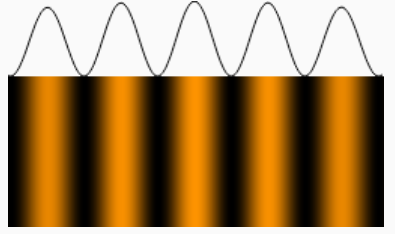
\includegraphics[scale=0.4]{Figures/coh_spatiale.png}
  }
  \subfigure[]{\label{fig:}
  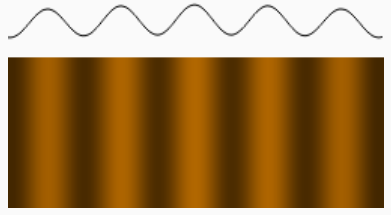
\includegraphics[scale=0.4]{Figures/perte_coh_spatiale.png}
  }
  \subfigure[]{\label{fig:}
  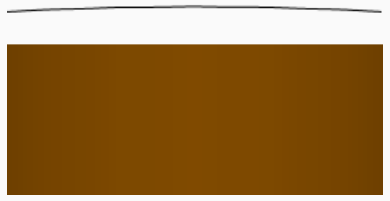
\includegraphics[scale=0.4]{Figures/perte_coh_spatiale_complete.png}
  }
  \caption{Perte de contraste global sur une figure d'interférences en raison de l'élargissement spatial de la source. (a) Source ponctuelle : la figure d'interférences est parfaitement contrastée. (b) Source étendue et $a < \ls$ : la figure d'interférences est moins contrastée. (c) Source étendue et $a \simeq \ls$ : la figure d'interférences est complètement brouillée. }
  \label{fig:}
\end{figure}
\begin{figure}[H]
  \centering
  \subfigure[]{\label{fig:source_fine}
  
\includegraphics[height=2.8cm]{source_fine.png}
  }
  \subfigure[]{\label{fig:source_moyenne}
  
\includegraphics[height=2.8cm]{source_moyenne.png}
  }
  \subfigure[]{\label{fig:source_large}
  
\includegraphics[height=2.8cm]{source_large.png}
  }
 \caption{Figure d'interférences en lumière blanche pour (a) une source peu étendue dans la direction des trous, (b) moyennement étendue, (c) très étendue. Le segment blanc à haut à gauche de chaque figure indique la taille de la source. On note la perte progressive de contraste qui affecte toute la figure d'interférences. Lien YouTube: \href{https://youtu.be/tc6V9B7YjtU}{\lcl{ici}}.}
 \label{fig:effet_largeur_source}
 \end{figure}


Ce cas est général à tous les interféromètres à division du front d'onde: la figure d'interférences se brouille très rapidement lorsqu'on utilise une source étendue dans la direction perpendiculaire à l'axe des trous (cohérence spatiale faible), ce qui est pourtant nécessaire pour obtenir une luminosité suffisante (même si c'est à nuancer depuis la découverte des lasers).

% \begin{remarque}
% Même si les terminologies sont proches, attention à ne pas confondre la perte de cohérence spatiale (causée par l'élargissement spatial de la source pour permettre une meilleure luminosité) avec la perte de cohérence temporelle étudiée au chapitre précédent (causée par l'élargissement spectral de la source, et qui dépend du processus d'émission de la lumière). Pour obtenir des interférences visibles, il faut que les deux conditions soient réunies: d'une part que les 2 ondes puissent interférer et donc que la différence de marche n'excède pas la longueur de cohérence temporelle $\delta<l_{\rm{c}}=\tfrac{\lambda^2}{\Delta\lambda}$; et d'autre part que la source ne soit pas trop étendue (cohérence spatiale) donc $2b<\tfrac{\lambda_0 d}{na}$, ce qui s'écrit aussi $a<l_{\rm{s}}=\tfrac{\lambda_0 d}{2bn}$ avec $a$ la distance entre les trous.
% \end{remarque}

\parag{Localisation des interférences}
Pour augmenter la luminosité de la figure d'interférences, il est important de pouvoir utiliser une source étendue, or nous venons de voir que cela peut conduire (si l'élargissement est parallèle à l'axe des trous) à un brouillage global de la figure d'interférences (perte de contraste). Mais existe-t-il une région spécifique du champ d'interférences plus propice à l'observation des interférences (où les franges sont mieux contrastées) ? Expérimentalement, on constate que cela n'est malheureusement pas le cas: on dit que les interférences sont \important{délocalisées}. On admettra qu'il s'agit d'une propriété générale de tous les interféromètres à division du front d'onde.

\begin{prop}[Interférences délocalisées]\label{prop:}
Les interférences issues de la division du front d'onde sont \important{délocalisées}. Elles sont visibles partout dans le champ d'interférences pour une source ponctuelle, mais brouillées partout pour une source étendue, ce qui empêche de former des figures d'interférences lumineuses.
\end{prop}

% Le (seul) point positif à cette non localisation est que les interférences sont observables en tout point du champ d'interférences\footnote{Par contre évidemment plus on éloigne l'écran des trous, moins la figure d'interférences observée est lumineuse puisque l'intensité de l'onde sphérique décroît comme $1/D^2$.}, ce qui facilite le réglage de l'interféromètre. Nous verrons dans le prochain chapitre que la situation est inversée pour les interféromètres à division d'amplitude, pour lesquels les interférences sont localisées avec une source étendue.

\begin{table}[h!] \centering
  \renewcommand{\arraystretch}{1.4}
  \begin{tabular}{|c|c|c|} \hline \textbf{Perte de cohérence...} & \textbf{temporelle} & \textbf{spatiale} \\ 
  \hline \hline 
  % Type de cohérence & Temporelle & Spatiale \\ 
  % \hline 
  Cause & Élargissement spectral (largeur $\Delta \lambda$) & Élargissement spatial (largeur $b$) \\ \hline
  Longueur caractéristique & $\lc \simeq \frac{\lambda^2}{\Delta \lambda}$ & $\ls \simeq \frac{\lambda d}{b}$ \\ \hline 
  Critère de cohérence & $\delta \lesssim \lc$ & $a \lesssim \ls$ \\ \hline 
  Effet & Brouillage local & Brouillage global \\ \hline 
  % Allure de l'intensité & 
  
\end{tabular} \caption{Propriétés des pertes de cohérence temporelle et spatiale.} \label{tab:proprietes} \end{table}






%Interprétons cette figure. La frange centrale correspond à $\delta=0$, superposition de toutes les couleurs, elle est donc blanche. Puis pour une différence de marche donnée $\delta$, les valeurs de $\lambda_0$ (les couleurs) telles que $p=\delta/\lambda_0$ est demi-entier sont absentes du spectre car elles donnent lieu à des interférences destructives.
%
% Au voisinage immédiat de la frange centrale, $\delta$ est très petit, typiquement \SI{1}{\micro\meter} ou moins, et une seule longueur d'onde est éteinte dans le visible. La teinte observée est alors la couleur complémentaire de la couleur éteinte. Ces teintes sont appelées \important{teintes de Newton}: leur couleur permet de déterminer précisément la différence de marche\footnote{L'échelle complète est disponible sur l'article Wikipédia \guill{Échelle des teintes de Newton}.}.
%
% \begin{figure}[h!]
% \centering
% 
\includegraphics[width=0.5\textwidth]{couleur-complémentaire.jpg}
% \caption{Les couleurs diamétralement opposées sont complémentaires.}
% \end{figure}
%
% En revanche lorsque $\delta$ devient plus important (typiquement à partir de \SI{3}{\micro\meter}), de nombreuses longueurs d'onde sont éteintes dans le spectre et l'intensité observée apparaît blanche à l’œil. Toutefois, cette couleur n'est pas de la lumière blanche, on l'appelle le \important{blanc d'ordre supérieur}. Son spectre est \important{cannelé}, c'est-à-dire qu'il présente des oscillations rapides de l'intensité avec des minima qui apparaissent noirs. Chaque cannelure représente une extinction où l'ordre d'interférences est demi-entier. Au delà de quelques (entre 3 et 6 selon les auteurs) cannelures dans le visible, notre œil perçoit seulement du blanc, mais ces cannelures sont observables à l'aide d'un spectromètre (Fig.~\ref{fig:cannelures}).
%  \begin{figure}[h!]
%  \centering
%  
\includegraphics[width=0.65\textwidth]{cannelures.pdf}
%  \caption{Cannelures du blanc d'ordre supérieur observées avec un spectromètre. Source: phitem.univ-grenoble-alpes.fr}
%  \label{fig:cannelures}
%  \end{figure}
%
% Compter le nombre de cannelures dans un certain intervalle de longueurs d'onde $\Delta\lambda$ peut permettre par exemple de réaliser des mesures très précises (épaisseur d'une lame ou de son indice optique par exemple, voir TD).
%
% \begin{remarque}
% Attention, un spectre cannelé n'est pas une figure d'interférences! En effet, il est créé par une superposition d'intensités lumineuses (et non pas d'amplitudes!) correspondant à des longueurs d'onde différentes. Tout se passe comme s'il y avait addition de multiples sources secondaires incohérentes.
% \end{remarque}



\section{Le réseau par transmission}
 Les trous de Young réalisent une interférence à deux ondes. Nous avons vu que la finesse d'un instrument augmente avec le nombre $N$ d'ondes qui interférent. Nous allons donc maintenant étudier un interféromètre à division du front d'ondes à $N$ ondes, le réseau de diffraction.
%  . Nous verrons que les interférences sont alors localisées, ce qui permet de former des figures d'interférences lumineuses. Nous étudierons dans un premier temps le réseau par transmission, puis le réseau par réflexion.
\subsection{Description}

\begin{definition}[Réseau de diffraction]\label{def:}
  Un \imp{réseau de diffraction} est un arrangement régulier de $N$ motifs diffractants identiques séparés par un intervalle $a$ appelé \imp{pas du réseau}.
  % , appelés \imp{fentes}, séparés par des intervalles transparents.
\end{definition}
% De manière générale, un réseau de diffraction est un arrangement régulier de motifs diffractants identiques. On distingue deux types de réseaux de diffraction :
% \begin{liste}
%   \item les réseaux de diffraction par \imp{transmission}, où les motifs sont des fentes transparentes séparées par des intervalles opaques;
%   \item les réseaux de diffraction par \imp{réflexion}, où les motifs sont des miroirs séparés par des intervalles transparents.
% \end{liste}
% Chaque motif diffracte la lumière incidente dans toutes les directions, et chaque faisceau diffracté dans une direction interfère avec les autres rayons diffractés dans la même direction.

Bien qu'il existe une grande diversité de formes (plane, concave), de types (rectiligne, circulaire) et de fonctionnement (en transmission, en réflexion), l'étude du réseau de fentes transparentes permet de dégager les propriétés essentielles des réseaux \Fig{reseau}. Il est réalisé en gravant sur du verre une série de traits à l'aide d'une pointe de diamant. L'espace intact entre ces traits est transparent et constitue une fente. En général, on réalise des répliques (diapositives photographiques) du réseau initial pour obtenir des réseaux à faible coût.
 Un réseau est caractérisé par le \imp{pas} du réseau, qui représente la distance $a$ entre deux fentes, ou le \imp{nombre de traits} par mm, qui vaut $1/a$. 
%   noté $n$, tel que
% \begin{equation}
%   n = \frac{1}{a}~(\SI{}{mm^{-1}}).
% \end{equation}
% À ne pas confondre avec l'indice optique $n$ (supposé valoir $1$ ici pour simplifier) !

\subsection{Figure d'interférences}


\begin{figure}[H]
  \centering
  \subfigure[]{\label{fig:reseau}
  
\includegraphics[width=0.45\textwidth]{reseaux-fentes.pdf}
  }
  \subfigure[]{
    
\includegraphics[width=0.45\textwidth]{réseau_transmission.pdf}
    }
  \caption{(a) Principe d'un réseau en transmission. Les fentes transparentes sont de largeur $\ell$ et séparées de $a$ : le pas du réseau. (b) Calcul de la différence de marche pour un réseau en transmission.}
  \end{figure}
  
  \parag{Ordres d'interférences observables}
On éclaire avec une lumière monochromatique parallèle un ensemble de $N$ fentes de Young identiques du réseau, équidistantes de $a$. Dans l'air d'indice $n\simeq 1$, la différence de marche entre deux fentes successives vaut
\begin{equation}
\delta=O_{m+1}J-KO_{m}=a\left(\sin(i')-\sin(i)\right).
\end{equation}
On observe des franges brillantes pour un ordre d'interférence $p=\frac{\delta}{\lambda_0}$ entier, c'est-à-dire
\begin{equation}
\label{eq:relation fondamentale du réseau}
\sin(i')-\sin(i)= p\frac{\lambda_0}{a}.
\end{equation}
Ce résultat se généralise à tout milieu homogène en remplaçant $\lambda_0$ par la longueur d'onde dans le milieu~$\lambda$.
\begin{theorem}[Formule des réseaux]\label{form:}
On observe une interférence \imp{constructive} dans toute direction $i'$ en sortie du réseau vérifiant
$$
\sin(i')-\sin(i)=p\frac{\lambda}{a}, \qquad p\text{ entier.}
$$
\end{theorem}
On observe un nombre fini d'ordres d'interférences parce que la fonction sinus est bornée. En effet, en incidence normale $i=0$, et $\abs{\sin(i')}\leq 1$, donc
% \begin{equation}
  \eqbox[]{
    \abs{p}\leq \frac{a}{\lambda}.
  }
La grandeur $\frac{a}{\lambda}$ donne l'ordre d'interférence maximal observable.   La construction géométrique de la Fig.~\ref{fig:interfs_reseau_incidence_normale} permet de visualiser les ordres d'interférences.
% \end{equation}

\begin{exemple}{Ordre d'interférence maximal observable}
  Déterminer l'ordre d'interférence maximal observable pour un réseau à $100$ traits par mm éclairé par un laser He-Ne de longueur d'onde $\lambda = \SI{632}{nm}$. 
  % Attention, si l'on se place , $\abs{\sin(i')-\sin(i)}\leq 1$ car $i=0$ et donc on a $\abs{p}\leq \frac{a}{\lambda_0}$.
\end{exemple}
\examplesol{
  On a $a=\SI{10}{\mu m}$ et donc $|p| < 16$.
}




\begin{figure}[h!]
\centering
\subfigure[]{

\includegraphics[width=0.48\textwidth]{ordres_reseau_construction.pdf}
}
\subfigure[]{\label{fig:Nondes}

\includegraphics[width=0.48\textwidth]{Nondes.pdf}
}
\caption{(a) Interférences constructives en incidence normale $(i=0)$. L'intersection avec le cercle de rayon $1$ permet de construire géométriquement les directions telles que $\sin(i')=p\lambda/a$. (b) Profil d'intensité en sortie d'un réseau par transmission en fonction du déphasage entre deux fentes successives $\varphi$ pour $N=4$. }
\label{fig:interfs_reseau_incidence_normale}
\end{figure}


\parag{Profil d'intensité}
Deux ondes produites par deux sources secondaires successives $O_{m}$ et $O_{m+1}$ sont déphasées de 
$$\varphi = 2\pi \frac{\delta}{\lambda_0} = 2\pi \left[\sin(i')-\sin(i)\right] \frac{a}{\lambda_0}.$$ Ce déphasage est indépendant de la source $O_m$ ! On peut donc utiliser la formule de l'intensité pour une interférences à $N$ ondes déphasées par un déphasage constant :
\begin{equation}
  I(\varphi)=\frac{I_{\rm{max}}}{N^2}\frac{\sin^{2}(N\varphi/2)}{\sin^{2}(\varphi/2)}.
\end{equation}
L'allure de cette fonction est rappelé en \Fig{Nondes}. On rappelle que l'intensité s'annule lorsque $\vphi = \frac{2m\pi}{N}$ avec $1\leq m \leq N-1$, ce qui correspond à un ordre d'interférence fractionnaire $p=\frac{m}{N}$.

%
% \parag{Minimum de déviation}
% On définit l'angle de déviation du réseau par $D=i'-i$, qui est une seule fonction de l'angle d'incidence $i$ puisque $i'$ est une fonction de $i$ et des paramètres du réseau d'après l'Éq.~\eqref{eq:relation fondamentale du réseau}.
% Au minimum de déviation on a
% \begin{equation}
% \frac{\d D}{\d i}=0=\frac{\d i'}{\d i}(i^{\star})-1.
% \end{equation}
% Or en dérivant l'Éq.~\eqref{eq:relation fondamentale du réseau}, il vient
% \begin{equation}
% \cos i' \,\d i' = \cos i \,\d i
% \end{equation}
% donc au minimum de déviation il faut avoir $\cos i'=\cos i$. Autrement dit ou bien $i'=i$ (ordre 0), ou bien $i'=-i$ (ordres supérieurs) et donc $D_{\rm{min}}=-2i$. La relation~\eqref{eq:relation fondamentale du réseau} devient donc au minimum de déviation
% \begin{equation}
% \label{eq:relation minimum de déviation}
% 2\sin\left(\frac{D_{\rm{min}}}{2}\right)=\frac{p\lambda_0}{a}.
% \end{equation}
%
% \parag{Utiliser le minimum de déviation avec un goniomètre}
% Il est possible de tirer profit de l'Éq.~\eqref{eq:relation minimum de déviation} pour mesurer à partir d'une mesure de l'angle de déviation réalisée au goniomètre une longueur d'onde inconnue $\lambda_0$. Un protocole possible est le suivant:
% \begin{figure}[h!]
% \centering
% 
\includegraphics[width=0.6\textwidth]{reseau_mesure_Dmin.pdf}
% \caption{Principe de mesure du minimum de déviation avec un réseau au goniomètre. Le plan du réseau est bissecteur du rayon incident et de la position du minimum de déviation, autrement dit les deux angles représentés en bleu sont égaux (et de même les deux angles en vert sont égaux pour la seconde position du réseau).}
% \end{figure}
% \begin{protocole}
% \item à l'aide d'un laser de longueur d'onde connue, on étalonne le dispositif afin de déterminer le pas du réseau $a$ (ou le nombre de traits par mm) si celui-ci n'est pas connu. Pour cela, on repère un ordre donné, et on mesure les deux positions angulaires $\theta_1$ et $\theta_2$ pour lesquelles la déviation observée est minimale en faisant tourner le plateau. Ensuite on calcule $2D_{\rm{min}}=\abs{\theta_1 - \theta_2}$. Enfin on répète l'opération pour plusieurs ordres afin d'améliorer la précision de la mesure.
% \item on tire profit du caractère fortement dispersif du réseau pour analyser une lumière inconnue et déterminer les longueurs d'onde de ses raies les plus intenses.
% \end{protocole}
% On notera que grâce à un nombre important de traits par mm, un réseau possède un fort pouvoir dispersif, bien meilleur que celui d'un prisme par exemple (voir TD et TP).
%


\bigskip
Pour clore ce chapitre, mentionnons qu'il existe d'autres dispositifs interférentiels par division du front d'onde (biprisme de Fresnel, miroirs de Fresnel, bilentilles de Billet ...). Ils s'analysent de la même manière que le dispositif de Young (détermination du champ d'interférences, calcul de la différence de marche, puis étude de la figure d'interférences avec expression de l'ordre d'interférences, de l'interfrange, du contraste etc.). Leur connaissance détaillée n'est pas au programme.


\end{document}
